\documentclass{beamer}
\usetheme{Singapore}
\usepackage{changepage}

%\usepackage{pstricks,pst-node,pst-tree}
\usepackage{amssymb,latexsym}
\usepackage{tikz}
\usepackage{graphicx}
\usepackage{fancyvrb}
\usepackage{hyperref}
\usepackage{fancybox}
\usepackage[listings]{tcolorbox}

\definecolor{codegreen}{rgb}{0,0.6,0}
\definecolor{codegray}{rgb}{0.5,0.5,0.5}
\definecolor{codepurple}{rgb}{0.58,0,0.82}
\definecolor{backcolour}{rgb}{0.95,0.95,0.92}

\lstdefinestyle{mystyle}{
    language=Python,
    backgroundcolor=\color{backcolour},   
    commentstyle=\color{codegreen},
    keywordstyle=\color{magenta},
    numberstyle=\tiny\color{codegray},
    stringstyle=\color{codepurple},
    basicstyle=\ttfamily\footnotesize,
    breakatwhitespace=false,         
    breaklines=true,                 
    captionpos=b,                    
    keepspaces=true,                 
    numbers=left,                    
    numbersep=5pt,                  
    showspaces=false,                
    showstringspaces=false,
    showtabs=false,                  
    tabsize=2,
    escapechar=|,
    frame=single
}

\lstset{style=mystyle}


\newcommand{\bi}{\begin{itemize}}
\newcommand{\li}{\item}
\newcommand{\ei}{\end{itemize}}
\newcommand{\Show}[1]{
\begin{center}
\shadowbox{\begin{minipage}{0.8\textwidth}
          #1
          \end{minipage}}
\end{center}
}
\newcommand{\arrow}{\ensuremath{\rightarrow}}

\newcommand{\uparr}{\ensuremath{\uparrow}}


\newcommand{\img}[2]{\centerline{\includegraphics[width=#1\textwidth]{#2}}}

\newcommand{\bfr}[1]{\begin{frame}[fragile]\frametitle{{ #1 }}}
\newcommand{\efr}{\end{frame}}

\newcommand{\cola}{\begin{columns}\begin{column}{0.5\textwidth}}
\newcommand{\colb}{\end{column}\begin{column}{0.5\textwidth}}
\newcommand{\colc}{\end{column}\end{columns}}


\title{Think Python 2e, Chapter 6 Notes}
\author{Geoffrey Matthews}

\begin{document}

\begin{frame}
\maketitle

\end{frame}

\bfr{Fruitful Functions}
\begin{lstlisting}
def area(radius):
    a = math.pi * radius**2
    return a
\end{lstlisting}
\pause
Return value can be complex:
\begin{lstlisting}
def area(radius):
    return math.pi * radius**2
\end{lstlisting}
But easier to debug with {\bf temporary variables}.
\end{frame}

\bfr{More than one return}
\begin{lstlisting}
def absolute_value(x):
    if x < 0:
        return -x
    else:
        return x
\end{lstlisting}
Only one return executes.
\pause

Make sure every possible path through the function
hits a return!
\begin{lstlisting}
def absolute_value(x):
    if x < 0:
        return -x
    if x > 0:
        return x
\end{lstlisting}
What does it return if \verb|x == 0|?
\end{frame}

\bfr{Incremental development}
\[ \mathit{distance} = \sqrt{(x_2-x_1)^2 + (y_2-y_1)^2} \]

Can immediately write:
\begin{lstlisting}
def distance(x1, x2, y1, y2):
	return 0.0
\end{lstlisting}
\pause

\begin{itemize}
\item
Not much, but at least it runs without error and
returns a value of the correct type.
\item
If this is part of a much larger program
that computes distances, does arithmetic with them,
prints them out, {\em etc.}
you can check the rest of the program without
finishing this part.
\end{itemize}


\end{frame}


\bfr{Incremental development}
\[ \mathit{distance} = \sqrt{(x_2-x_1)^2 + (y_2-y_1)^2} \]

Start adding some intermediate values:
\begin{lstlisting}
def distance(x1, y1, x2, y2):
    dx = x2 - x1
    dy = y2 - y1
    print('dx is', dx)
    print('dy is', dy)
    return 0.0
\end{lstlisting}


\begin{itemize}
\item
Develop a test case, where you know the answer.
\item For example: \verb|distance(0, 0, 3, 4)|
\item I know this is 5 because a 3,4,5 triangle is a right
triangle.
\item
Testing the above we can make sure that \verb|dx| is 3
and \verb|dy| is 4
\end{itemize}


\end{frame}

\bfr{Incremental development}
\[ \mathit{distance} = \sqrt{(x_2-x_1)^2 + (y_2-y_1)^2} \]

Add some more code:
\begin{lstlisting}
def distance(x1, y1, x2, y2):
    dx = x2 - x1
    dy = y2 - y1
    dsquared = dx**2 + dy**2
    print('dsquared is: ', dsquared)
    return 0.0
\end{lstlisting}
Test it.
\end{frame}

\bfr{Incremental development}
\[ \mathit{distance} = \sqrt{(x_2-x_1)^2 + (y_2-y_1)^2} \]

Finally, add the last bit of code:
\begin{lstlisting}
def distance(x1, y1, x2, y2):
    dx = x2 - x1
    dy = y2 - y1
    dsquared = dx**2 + dy**2
    result = math.sqrt(dsquared)
    return result
\end{lstlisting}
Test this.  If all is well, we're done.

Using intermediate variables allows us test each step.

such print statements are called {\bf scaffolding}.

\end{frame}

\bfr{Alternative strategy: dead code}
\cola
\begin{lstlisting}
def distance(x1,y1, x2,y2):
    return 5;
    dx = x2 - x1
    dy = y2 - y1
    dsq = dx**2+dy**2
    result = math.sqrt(dsq)
    return result
\end{lstlisting}\pause
\begin{lstlisting}
def distance(x1,y1, x2,y2):
    dx = x2 - x1
    return dx
    dy = y2 - y1
    dsq = dx**2+dy**2
    result = math.sqrt(dsq)
    return result
\end{lstlisting}\pause
\colb
\begin{lstlisting}
def distance(x1,y1, x2,y2):
    dx = x2 - x1
    dy = y2 - y1
    return dy
    dsq = dx**2+dy**2
    result = math.sqrt(dsq)
    return result
\end{lstlisting}\pause
\begin{lstlisting}
def distance(x1,y1, x2,y2):
    dx = x2 - x1
    dy = y2 - y1
    dsq = dx**2+dy**2
    return dsq
    result = math.sqrt(dsq)
    return result
\end{lstlisting}
\colc

\end{frame}

\bfr{Debugging modules}

\begin{lstlisting}
import math

def distance(x1, y1, x2, y2):
    dx = x2 - x1
    dy = y2 - y1
    dsquared = dx**2 + dy**2
    result = math.sqrt(dsquared)
    return result    

# The following code will be run if this module is run
# It will NOT be run if the module is imported
if __name__ == '__main__':
    print(distance(0,0,3,4), 'should be', 5)
    print(distance(3,4,0,0), 'should be', 5)
    print(distance(1,1,4,5), 'should be', 5)
    print(distance(0,0,6,8), 'should be', 10)
\end{lstlisting}


\end{frame}

\bfr{Boolean functions}
\begin{lstlisting}
def is_divisible(x, y):
    if x % y == 0:
        return True
    else:
        return False
\end{lstlisting}

Frequently given names that sound like 
yes/no questions and their answers:
\begin{itemize}
\item Is \verb|x| divisible by \verb|y|?
\item Yes, \verb|x| is divisible by \verb|y|.
\end{itemize}

\begin{lstlisting}
>>> is_divisible(6, 4)
False
>>> is_divisible(6, 3)
True
\end{lstlisting}


\end{frame}


\bfr{Boolean functions}
Frequently boolean functions
can be shortened:

\begin{lstlisting}
def is_divisible(x, y):
    if x % y == 0:
        return True
    else:
        return False
\end{lstlisting}

\begin{lstlisting}
def is_divisible(x, y):
    return x % y == 0
\end{lstlisting}
\end{frame}

\bfr{Circular definitions}

\begin{description}
\item[vorpal:] an adjective used to define something
that is vorpal.
\end{description}

\end{frame}

\bfr{Recursive definitions}
\begin{description}
\item[vorpal:] an adjective applying to either:
\begin{itemize} 
\item a cat
\item a dog
\item a box containing something vorpal
\end{itemize}
\end{description}

\end{frame}

\bfr{Recursive functions}
\[
n! = \left\{ \begin{array}{ll}
              1 & \mbox{if $n = 0$} \\
              n(n-1)! & \mbox{if $n >  0$} \\
              \mbox{\it undefined} & \mbox{otherwise}
              \end{array}\right.
              \]
              
\[ 5! = 5\cdot 4\cdot 3\cdot 2\cdot 1 \cdot 1 = 120\]
\pause
\begin{lstlisting}
def factorial(n):
    if n < 0:
        return None
    elif n == 0:
        return 1
    else:
        return n * factorial(n - 1)
\end{lstlisting}
\end{frame}


\bfr{Recursive functions}
\begin{lstlisting}
def factorial(n):
    if n == 0:
        return 1
    else:
        recurse = factorial(n-1)
        result = n * recurse
        return result
\end{lstlisting}
\begin{lstlisting}
factorial(3)
\end{lstlisting}
{\tt
\begin{tabular}{|rccc||l|}\hline
\_\_main\_\_ &&&&\\\hline
factorial & n\arrow 3 & recurse\arrow 2 & result\arrow 6 & \uparr 6 \\\hline\hline
factorial &  n\arrow 2 & recurse\arrow 1 & result\arrow 2 & \uparr  2\\\hline\hline
factorial &  n\arrow 1 & recurse\arrow 1 & result\arrow 1 & \uparr 1 \\\hline\hline
factorial &  n\arrow 0 &  &  & \uparr 1\\\hline
\end{tabular}
}
\end{frame}

\bfr{Fibonacci numbers}
\[
\mathit{fibonacci}(n) = \left\{
  \begin{array}{ll}
    0 & \mbox{if $n = 0$}\\
    1 & \mbox{if $n = 1$}\\
    \mathit{fibonacci}(n-1) + \mathit{fibonacci}(n-1) & \mbox{otherwise}
    \end{array}\right.
\]
\[0, 1, 1, 2, 3, 5, 8, 13, 21, 34, 55, 89, 144, 233, 377, 610, 987, ...
\]
\begin{lstlisting}
def fibonacci(n):
    if n == 0:
        return 0
    elif  n == 1:
        return 1
    else:
        return fibonacci(n-1) + fibonacci(n-2)
\end{lstlisting}
\end{frame}

\bfr{Checking arguments}
\begin{lstlisting}
def factorial(n):
    if n == 0:
        return 1
    else:
        return n * factorial(n - 1)
\end{lstlisting}
\begin{lstlisting}
>>> factorial(1.5)
RuntimeError: Maximum recursion depth exceeded
>>> factorial(-3)
RuntimeError: Maximum recursion depth exceeded
\end{lstlisting}


\end{frame}

\bfr{Checking arguments}
\begin{lstlisting}
def factorial(n):
    if not isinstance(n, int):
        print('Factorial is only defined for integers.')
        return None
    elif n < 0:
        print('Factorial is not defined for negative integers.')
        return None
    elif n == 0:
        return 1
    else:
        return n * factorial(n-1)
\end{lstlisting}

The two conditionals that return \verb|None|
are called {\bf guardians}.


\end{frame}

\bfr{Vocabulary}
\begin{description}

\li[temporary variable:]
A variable used to store an intermediate value in a complex calculation.
\li[dead code:]
Part of a program that can never run, often because it appears after a return statement.
\li[incremental development:]
A program development plan intended to avoid debugging by adding and testing only a small amount of code at a time.
\li[scaffolding:]
Code that is used during program development but is not part of the final version.
\li[guardian:]
A programming pattern that uses a conditional statement to check for and handle circumstances that might cause an error.
\end{description}
\end{frame}

\begin{frame}

\frametitle{Ackermann function}
\[
  A(x,y) = \left\{\begin{array}{ll}y+1 & \mbox{if\ } x = 0\\
                                A(x-1,1) & \mbox{if\ } y=0\\
                                A(x-1,A(x,y-1)) &\mbox{otherwise}
                   \end{array}\right.
\]

\pause
\bigskip

\hspace*{-0.35in}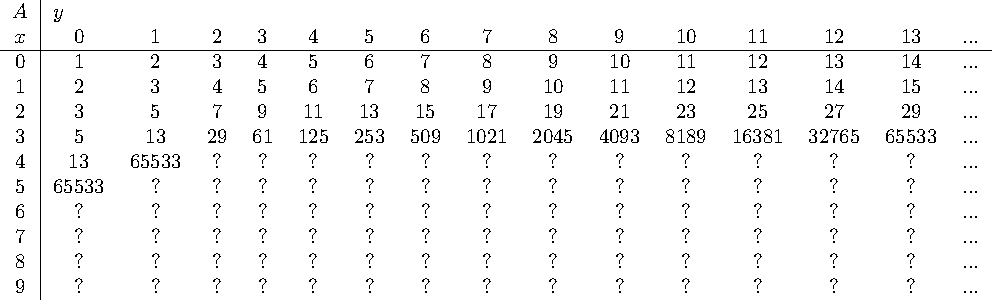
\includegraphics[width=5in]{ackermann.pdf}

\end{frame}

\end{document}
